\documentclass[conference]{IEEEtran}
\IEEEoverridecommandlockouts
\usepackage{amsmath,amssymb}
\usepackage{graphicx}
\usepackage{cite}
\usepackage{hyperref}
\usepackage{booktabs}
\usepackage{listings}
\usepackage{xcolor}
\usepackage{pgfplots}
\pgfplotsset{compat=1.17}

\lstset{
  basicstyle=\ttfamily\small,
  breaklines=true,
  columns=fullflexible,
  backgroundcolor=\color{gray!10},
  frame=single
}

\title{tinyGPT: A From-Scratch C++ Implementation of a Character-Level Transformer with Hand-Derived Backpropagation}

\author{
\IEEEauthorblockN{Shivansh Pratap Singh\thanks{Corresponding author: Shivansh Pratap Singh (email: cse23308@glbitm.ac.in).}}
\IEEEauthorblockA{Department of Computer Science and Engineering\\
G. L. Bajaj Institute of Technology and Management\\
Plot No. 2, Knowledge Park III, Greater Noida, Uttar Pradesh 201306, India\\
Email: cse23308@glbitm.ac.in}
}

\begin{document}

\maketitle

\begin{abstract}
We present tinyGPT, a character-level transformer language model implemented entirely from scratch in C++ with no machine learning or linear algebra libraries. The forward pass, backward pass, and optimizer are hand-derived on top of a small self-built matrix autograd engine. We describe two implementations: a minimal single-head, single-block model (tinygpt) and an extended version (tinygpt2) with multi-head attention, two stacked transformer blocks, and Pre-LayerNorm. Both are trained on a character-level corpus using the Adam optimizer with causal masking. We report training loss curves and generated samples for both models trained on \textit{Alice's Adventures in Wonderland}, showing that the architectural extensions in tinygpt2 reduce final training loss from 1.77 to 1.59 at comparable iteration counts, and to 1.40 with extended training. We discuss implementation details including a reference-cycle memory bug in the autograd engine, learning rate sensitivity, and the empirical decision to omit LayerNorm in the single-block model. The project's goal is pedagogical: to understand attention and backpropagation through direct implementation rather than to produce a competitive language model.
\end{abstract}

\begin{IEEEkeywords}
transformer, attention mechanism, autograd, backpropagation, character-level language model, C++
\end{IEEEkeywords}

\section{Introduction}
Transformer-based language models are almost universally built on top of established deep learning frameworks such as PyTorch or TensorFlow, which abstract away the mechanics of automatic differentiation, tensor operations, and gradient computation. This abstraction is useful for building large-scale systems but obscures the underlying mathematics for anyone trying to understand \textit{how} a transformer actually computes its forward and backward passes.

tinyGPT is a character-level transformer written entirely in C++ using only the standard library. There is no autograd framework, no BLAS or linear algebra library, and no use of any external machine learning tooling. Every tensor operation, its corresponding backward rule, and the optimizer update are implemented by hand. The project is deliberately small in scale; it is not intended to compete with production language models but to serve as a complete, inspectable reference implementation of the components that make a transformer work: token and positional embeddings, causal self-attention, feedforward layers, LayerNorm, cross-entropy loss, and Adam optimization.

Two versions of the model are presented. tinygpt is the minimal version: a single attention head operating over the full embedding dimension, one transformer block, and no LayerNorm. tinygpt2 extends this into a more standard architecture: four attention heads, two stacked transformer blocks, and Pre-LayerNorm applied before each sub-layer. Both models share the same underlying autograd engine and are trained identically, which allows for a controlled comparison of how these architectural choices affect training loss and generated text quality.

\section{Related Work}
The transformer architecture was introduced for sequence modeling \cite{vaswani2017attention} and forms the basis of modern language models such as the GPT family \cite{radford2019gpt2}, which stack many transformer blocks with multi-head self-attention and LayerNorm to achieve high capacity language modeling. Educational reimplementations of GPT-style models exist in Python using minimal frameworks, typically still relying on PyTorch's autograd for gradient computation \cite{karpathy2022nanogpt}. tinyGPT differs from these in that it does not use any autograd framework at all; the computation graph, topological sort, and backward pass are all implemented manually in C++, and the only tensor abstraction is a simple 2D matrix with a forward value buffer and a gradient buffer.

\section{Autograd Engine}
The core of tinyGPT is a minimal reverse-mode automatic differentiation engine built around a single \texttt{Tensor} struct:

\begin{lstlisting}[language=C++]
struct Tensor {
    int r, c;
    vector<double> d, g;
    vector<TPtr> prev;
    function<void()> bw;
};
\end{lstlisting}

Each tensor stores its forward values (\texttt{d}), accumulated gradients (\texttt{g}), a list of parent tensors (\texttt{prev}), and a backward closure (\texttt{bw}) that routes gradients to its parents. Every operation constructs a new output tensor, records its parents, and attaches a lambda that implements the operation's backward rule. Calling \texttt{backward()} on a loss tensor performs a topological sort over the graph reachable from the loss, initializes the loss gradient to 1.0, and walks the sorted order in reverse, invoking each tensor's backward closure.

A notable implementation issue arose from how backward closures captured their own output tensor. Capturing a \texttt{shared\_ptr} to the tensor itself inside its own backward lambda creates a reference cycle: the tensor's \texttt{bw} closure holds a shared pointer to the tensor, and the tensor holds the closure, so neither is ever freed. This caused memory to grow unbounded during training until the process was killed by the operating system. The fix was to capture a raw pointer (\texttt{Tensor* op = o.get()}) instead of the shared pointer, breaking the cycle while relying on the caller holding the owning \texttt{shared\_ptr} to keep the tensor alive for the duration it is needed.

Table~\ref{tab:ops} lists the tensor operations implemented, along with their backward rules.

\begin{table}[h]
\centering
\caption{Autograd Operations}
\label{tab:ops}
\begin{tabular}{ll}
\toprule
Operation & Backward Rule \\
\midrule
matmul(A, B) & $dA \mathrel{+}= dO \, B^\top,\ dB \mathrel{+}= A^\top dO$ \\
add(a, b) & $da \mathrel{+}= dO,\ db \mathrel{+}= dO$ \\
add\_bias(a, b) & $db$ = column-wise sum of $dO$ \\
relu(a) & $da \mathrel{+}= dO \cdot \mathbb{1}[a>0]$ \\
scale(a, s) & $da \mathrel{+}= dO \cdot s$ \\
transpose(a) & $da[i,j] \mathrel{+}= dO[j,i]$ \\
causal\_mask(a) & pass-through on lower triangle \\
softmax\_rows(a) & Jacobian via dot-product trick \\
embed(E, idx) & scatter-add into embedding rows \\
concat\_cols(ts) & slice gradient back per input \\
layernorm\_rows & standard LN backward formula \\
\bottomrule
\end{tabular}
\end{table}

\section{Model Architecture}

\subsection{tinygpt}
The baseline model processes a sequence of $T$ character indices through a single attention head and a single transformer block:

\begin{align}
x &= \text{Embed}(E, \text{idx}) + P[:T] \\
Q, K, V &= xW_q,\ xW_k,\ xW_v \\
\text{scores} &= \frac{QK^\top}{\sqrt{d}} \\
\text{attn} &= \text{softmax}(\text{causal\_mask}(\text{scores})) \\
x &= x + (\text{attn} \cdot V) W_o \\
x &= x + \text{ReLU}(xW_1 + b_1)W_2 + b_2 \\
\text{logits} &= xW_{\text{out}} + b_{\text{out}}
\end{align}

with $d=64$, feedforward hidden size $d_{ff}=256$, and context length (block) 64. No LayerNorm is used. The choice to omit LayerNorm was empirical rather than an oversight: it was implemented, its backward pass verified against a numerical gradient check, but it converged more slowly than the version without it at this scale. LayerNorm's benefit is primarily in stabilizing gradients across many stacked blocks; with a single block and a small dataset it adds optimization friction without a corresponding benefit.

\subsection{tinygpt2}
tinygpt2 extends the baseline with multi-head attention, two stacked transformer blocks, and Pre-LayerNorm applied before each sub-layer \cite{ba2016layernorm}:

\begin{equation}
x = x + \text{MHA}(\text{LN}(x)), \qquad x = x + \text{FFN}(\text{LN}(x))
\end{equation}

Each of the $n_h=4$ heads operates in $d_{\text{head}} = d/n_h = 16$ dimensions:

\begin{align}
Q_h, K_h, V_h &= xW_{q_h},\ xW_{k_h},\ xW_{v_h} \\
\text{attn}_h &= \text{softmax}\left(\text{causal\_mask}\left(\frac{Q_hK_h^\top}{\sqrt{d_{\text{head}}}}\right)\right) \\
\text{head}_h &= \text{attn}_h V_h
\end{align}

The per-head outputs are joined column-wise and projected back to the model dimension:

\begin{equation}
\text{out} = \text{concat\_cols}(\text{head}_0, \ldots, \text{head}_{n_h-1})\, W_o
\end{equation}

This requires a new autograd primitive, \texttt{concat\_cols}, whose backward pass slices the incoming gradient back into each head's gradient buffer according to its column offset.

Pre-LN is implemented as a second new primitive, \texttt{layernorm\_rows}, normalizing each row independently:

\begin{equation}
y_{i,j} = \gamma_j \cdot \frac{x_{i,j}-\mu_i}{\sigma_i} + \beta_j
\end{equation}

The backward pass with respect to the input is

\begin{equation}
\frac{\partial L}{\partial x_{i,j}} = \frac{1}{\sigma_i}\left(\widehat{dx}_{i,j} - \frac{1}{d}\sum_k \widehat{dx}_{i,k} - \hat{x}_{i,j}\cdot\frac{1}{d}\sum_k \widehat{dx}_{i,k}\hat{x}_{i,k}\right)
\end{equation}

where $\widehat{dx}_{i,j} = \frac{\partial L}{\partial y_{i,j}}\gamma_j$ and $\hat{x}_{i,j}$ is the normalized pre-scale value cached during the forward pass. The gradients with respect to $\gamma$ and $\beta$ are $\sum_i \frac{\partial L}{\partial y_{i,j}}\hat{x}_{i,j}$ and $\sum_i \frac{\partial L}{\partial y_{i,j}}$ respectively.

Table~\ref{tab:archcompare} summarizes the architectural differences between the two models.

\begin{table}[h]
\centering
\caption{Architecture Comparison}
\label{tab:archcompare}
\begin{tabular}{lll}
\toprule
Feature & tinygpt & tinygpt2 \\
\midrule
Attention heads & 1 ($d=64$) & 4 ($d_{\text{head}}=16$) \\
Transformer blocks & 1 & 2 \\
LayerNorm & none & Pre-LN \\
Parameter tensors & 12 & 48 \\
Iterations & 8000 & 10000 \\
Learning rate & 0.0025 & 0.001 \\
\bottomrule
\end{tabular}
\end{table}

\section{Training}
Both models are trained on character-level tokenization, where the vocabulary is simply the set of unique characters in the training corpus. Training minimizes cross-entropy loss, fused with softmax for numerical stability:

\begin{equation}
\mathcal{L} = -\frac{1}{T}\sum_{t=1}^{T} \log p_{t,y_t}, \qquad p_{t,j} = \text{softmax}(\text{logits}_t)_j
\end{equation}

with backward rule $\frac{\partial \mathcal{L}}{\partial \text{logit}_{t,j}} = \frac{1}{T}(p_{t,j} - \mathbb{1}[j=y_t])$.

Parameters are updated with Adam \cite{kingma2015adam} using standard bias-corrected moment estimates ($\beta_1=0.9$, $\beta_2=0.999$, $\epsilon=10^{-8}$). Each iteration samples a random contiguous window of length \texttt{block} from the corpus, computes the forward pass and loss, backpropagates, and applies an Adam step. Learning rate proved to be the most sensitive hyperparameter: a rate of 0.005 produced a visible loss spike mid-training at larger model sizes, while dropping to 0.0025 (tinygpt) or 0.001 (tinygpt2) eliminated the spike with no other changes.

At generation time, both models sample autoregressively at temperature 0.8, which sharpens the softmax distribution over the vocabulary relative to unscaled sampling.

\section{Results}
Both models were trained on \textit{Alice's Adventures in Wonderland} (approximately 50 KB, 64 unique characters) with a fixed random seed of 42. Table~\ref{tab:loss} reports training loss at selected iterations for tinygpt (8k iterations) and tinygpt2 (10k iterations), and Fig.~\ref{fig:loss8k10k} shows the corresponding loss curves.

\begin{table}[h]
\centering
\caption{Training Loss Comparison (8k vs 10k)}
\label{tab:loss}
\begin{tabular}{lcc}
\toprule
Iter & tinygpt (8k) & tinygpt2 (10k) \\
\midrule
1000 & 2.44 & 2.43 \\
3000 & 2.20 & 2.14 \\
5000 & 1.99 & 1.92 \\
7000 & 1.83 & 1.68 \\
8000 & 1.77 & 1.64 \\
10000 & --- & 1.59 \\
\bottomrule
\end{tabular}
\end{table}

\begin{figure}[h]
\centering
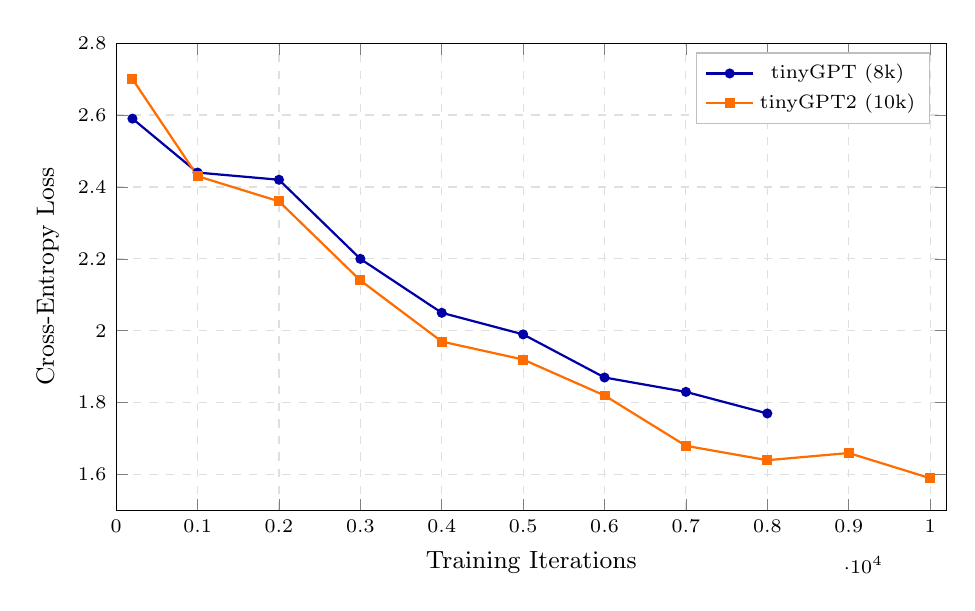
\begin{tikzpicture}
\begin{axis}[
    width=\columnwidth,
    height=0.62\columnwidth,
    xlabel={Training Iterations},
    ylabel={Cross-Entropy Loss},
    xmin=0, xmax=10200,
    ymin=1.5, ymax=2.8,
    grid=major,
    grid style={dashed, gray!25},
    label style={font=\small},
    tick label style={font=\scriptsize},
    legend style={font=\scriptsize, at={(0.98,0.98)}, anchor=north east, draw=gray!50},
    every axis plot/.append style={thick},
]
\addplot[color=blue!65!black, mark=*, mark size=1.4pt] coordinates {
(200,2.590) (1000,2.440) (2000,2.420) (3000,2.200) (4000,2.050) (5000,1.990) (6000,1.870) (7000,1.830) (8000,1.770)
};
\addlegendentry{tinyGPT (8k)}
\addplot[color=orange!85!red, mark=square*, mark size=1.4pt] coordinates {
(200,2.700) (1000,2.430) (2000,2.360) (3000,2.140) (4000,1.970) (5000,1.920) (6000,1.820) (7000,1.680) (8000,1.640) (9000,1.660) (10000,1.590)
};
\addlegendentry{tinyGPT2 (10k)}
\end{axis}
\end{tikzpicture}
\caption{Cross-entropy training loss versus training iterations for tinygpt (8k iterations, final loss 1.77) and tinygpt2 (10k iterations, final loss 1.59).}
\label{fig:loss8k10k}
\end{figure}

tinygpt reaches a final loss of 1.77 at 8000 iterations. tinygpt2 reaches 1.59 at 10000 iterations, already below tinygpt's loss at a comparable point in training, as summarized in Table~\ref{tab:loss8k10ksummary}.

Continuing tinygpt2's training run to 20000 iterations brings the loss down further, to 1.40 at 20000 iterations, with a best checkpoint of 1.342 reached at iteration 18{,}800 before the loss ticks back up slightly by iteration 20000. Table~\ref{tab:loss8k10ksummary} and Fig.~\ref{fig:loss20k} report this extended run alongside the original 8k/10k results.

\begin{table}[h]
\centering
\caption{Training Loss Comparison Summary}
\label{tab:loss8k10ksummary}
\begin{tabular}{lccc}
\toprule
Iter & tinygpt (8k) & tinygpt2 (10k) & tinygpt2 ext. (20k) \\
\midrule
1000 & 2.44 & 2.43 & 2.43 \\
3000 & 2.20 & 2.14 & 2.06 \\
5000 & 1.99 & 1.92 & 1.89 \\
7000 & 1.83 & 1.68 & 1.68 \\
8000 & 1.77 & 1.64 & 1.64 \\
10000 & --- & 1.59 & 1.59 \\
12000 & --- & --- & 1.56 \\
14000 & --- & --- & 1.51 \\
16000 & --- & --- & 1.42 \\
18000 & --- & --- & 1.39 \\
18800 & --- & --- & \textbf{1.34} (best) \\
20000 & --- & --- & 1.40 \\
\bottomrule
\end{tabular}
\end{table}

\begin{figure}[h]
\centering
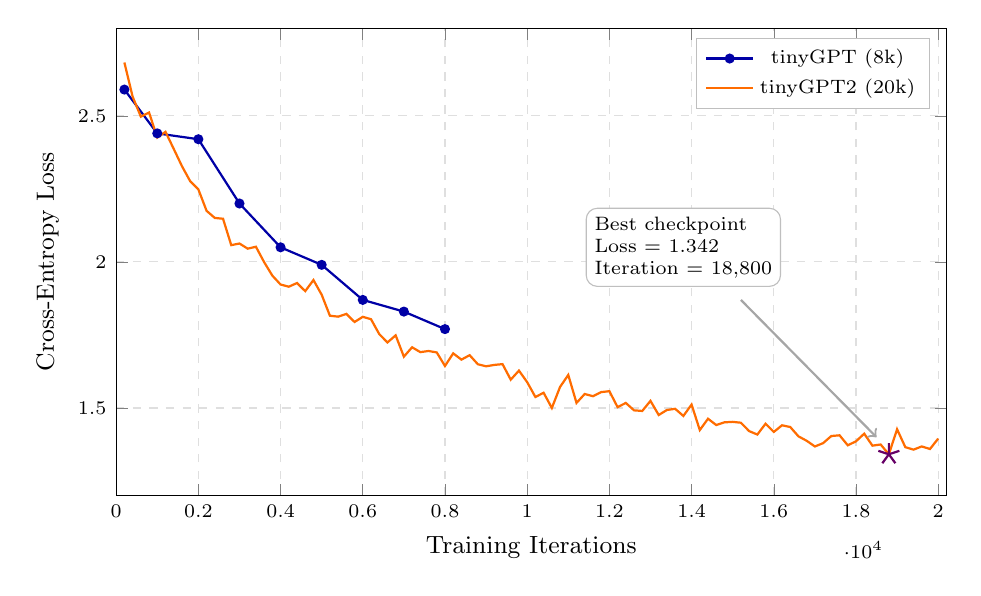
\begin{tikzpicture}
\begin{axis}[
    width=\columnwidth,
    height=0.62\columnwidth,
    xlabel={Training Iterations},
    ylabel={Cross-Entropy Loss},
    xmin=0, xmax=20200,
    ymin=1.2, ymax=2.8,
    grid=major,
    grid style={dashed, gray!25},
    label style={font=\small},
    tick label style={font=\scriptsize},
    legend style={font=\scriptsize, at={(0.98,0.98)}, anchor=north east, draw=gray!50},
    every axis plot/.append style={thick},
]
\addplot[color=blue!65!black, mark=*, mark size=1.4pt] coordinates {
(200,2.590) (1000,2.440) (2000,2.420) (3000,2.200) (4000,2.050) (5000,1.990) (6000,1.870) (7000,1.830) (8000,1.770)
};
\addlegendentry{tinyGPT (8k)}
\addplot[color=orange!85!red, mark=none] coordinates {
(200,2.68272) (400,2.56584) (600,2.49746) (800,2.51140) (1000,2.42573) (1200,2.44529) (1400,2.38706) (1600,2.32788) (1800,2.27655) (2000,2.24824) (2200,2.17487) (2400,2.15058) (2600,2.14778) (2800,2.05737) (3000,2.06302) (3200,2.04541) (3400,2.05197) (3600,1.99926) (3800,1.95308) (4000,1.92263) (4200,1.91520) (4400,1.92775) (4600,1.89995) (4800,1.93799) (5000,1.88772) (5200,1.81592) (5400,1.81267) (5600,1.82213) (5800,1.79442) (6000,1.81205) (6200,1.80397) (6400,1.75313) (6600,1.72431) (6800,1.74871) (7000,1.67570) (7200,1.70784) (7400,1.69119) (7600,1.69514) (7800,1.69018) (8000,1.64374) (8200,1.68704) (8400,1.66555) (8600,1.68074) (8800,1.64975) (9000,1.64267) (9200,1.64744) (9400,1.65017) (9600,1.59700) (9800,1.62798) (10000,1.58842) (10200,1.53762) (10400,1.55216) (10600,1.50007) (10800,1.57209) (11000,1.61319) (11200,1.51734) (11400,1.54795) (11600,1.54030) (11800,1.55439) (12000,1.55755) (12200,1.50293) (12400,1.51730) (12600,1.49194) (12800,1.48985) (13000,1.52443) (13200,1.47602) (13400,1.49320) (13600,1.49728) (13800,1.47274) (14000,1.51173) (14200,1.42441) (14400,1.46325) (14600,1.44166) (14800,1.45089) (15000,1.45254) (15200,1.44955) (15400,1.42093) (15600,1.40910) (15800,1.44620) (16000,1.41800) (16200,1.44077) (16400,1.43492) (16600,1.40298) (16800,1.38778) (17000,1.36828) (17200,1.37966) (17400,1.40407) (17600,1.40649) (17800,1.37239) (18000,1.38581) (18200,1.41207) (18400,1.37110) (18600,1.37504) (18800,1.34158) (19000,1.42723) (19200,1.36595) (19400,1.35742) (19600,1.36841) (19800,1.35962) (20000,1.39518)
};
\addlegendentry{tinyGPT2 (20k)}
\addplot[only marks, mark=star, mark size=4pt, color=violet!80!black] coordinates {(18800,1.34158)};
\node[align=left, font=\scriptsize, fill=white, draw=gray!50, rounded corners, inner sep=3pt] at (axis cs:13800,2.05) {Best checkpoint\\Loss = 1.342\\Iteration = 18{,}800};
\draw[->, thick, gray!70] (axis cs:15200,1.87) -- (axis cs:18500,1.40);
\end{axis}
\end{tikzpicture}
\caption{Extended training loss curve for tinygpt2 out to 20000 iterations, with the best checkpoint (loss = 1.342, iteration = 18{,}800) marked; tinygpt (8k) shown for reference.}
\label{fig:loss20k}
\end{figure}

Generated samples reflect this gap qualitatively. At loss 1.77, tinygpt produces mostly short fragments with scattered punctuation. At loss 1.59, tinygpt2 produces longer correctly spelled words (``little'', ``crown'', ``frown'', ``voices'', ``found'') and short multi-word phrases (``a little crown a frown'', ``Alice and her''). At loss 1.40 (20000 iterations), tinygpt2 produces recognizable multi-word structure and more natural punctuation placement, though the output remains far from grammatically coherent, consistent with the model's small scale (a two-block, 64-dimensional architecture on a small corpus).

Table~\ref{tab:params} shows the parameter tensor count growth from tinygpt to tinygpt2, driven by the four independent Q/K/V projections per head across two blocks plus the added LayerNorm scale/shift parameters.

\begin{table}[h]
\centering
\caption{Parameter Tensor Count}
\label{tab:params}
\begin{tabular}{lcc}
\toprule
Model & Parameter Tensors & Runtime (approx.) \\
\midrule
tinygpt & 12 & 2 min (8k iters) \\
tinygpt2 & 48 & 4 min (10k iters) \\
tinygpt2 (20k) & 48 & 8 min (20k iters) \\
\bottomrule
\end{tabular}
\end{table}

\section{Discussion}
The loss reduction from tinygpt to tinygpt2 (1.77 to 1.59 at comparable training budgets) is consistent with the expected effect of multi-head attention and Pre-LN: splitting the representation into multiple heads lets the model attend to different positional patterns in parallel, while Pre-LN stabilizes gradient flow through the two stacked residual paths. The fact that tinygpt2's loss curve had not plateaued at 10000 iterations, and continued improving meaningfully to a best checkpoint loss of 1.342 at iteration 18{,}800 (1.40 by iteration 20000), suggests the deeper architecture has more headroom to exploit than the single-block model, which is expected since additional depth increases model capacity relative to a fixed, small corpus.

The decision to omit LayerNorm in tinygpt is a useful negative result: LayerNorm did not fail to help because of an implementation bug — it was verified correct via numerical gradient checking — but because its main benefit (stabilizing gradients across many stacked normalization boundaries) does not manifest with only one block. This matches the standard understanding of why deep transformer stacks rely on normalization while very shallow ones can do without it.

\section{Conclusion}
tinyGPT demonstrates that a character-level transformer, including its full forward pass, hand-derived backward pass, and Adam optimizer, can be implemented from scratch in C++ without any machine learning or linear algebra dependencies. The comparison between a minimal single-head, single-block model and an extended multi-head, two-block, Pre-LN model shows a clear and expected improvement in training loss and generated text quality, validating that the hand-implemented multi-head attention and LayerNorm backward passes are correct and functioning as intended. Natural extensions include increasing model width ($d=128$), stacking additional blocks (3--4), and training on larger corpora, all of which the modular \texttt{Block}-based design in tinygpt2 supports without changes to the forward pass logic.

\section*{Acknowledgment}
The author used Claude (Anthropic) \cite{anthropic2026claude} to assist with reformatting and language editing of the manuscript text to improve clarity and ensure adherence to IEEE formatting guidelines. AI assistance was also used during development of the underlying tinyGPT/tinygpt2 C++ implementation for code cleanup, debugging, and identification of memory usage issues; the model design, hand-derived backpropagation rules, and all reported experiments and results are the author's own work.

\begin{thebibliography}{00}
\bibitem{vaswani2017attention} A. Vaswani, N. Shazeer, N. Parmar, J. Uszkoreit, L. Jones, A. N. Gomez, L. Kaiser, and I. Polosukhin, ``Attention is all you need,'' in \textit{Advances in Neural Information Processing Systems (NeurIPS)}, 2017, pp. 5998--6008.
\bibitem{radford2019gpt2} A. Radford, J. Wu, R. Child, D. Luan, D. Amodei, and I. Sutskever, ``Language models are unsupervised multitask learners,'' \textit{OpenAI Technical Report}, 2019.
\bibitem{karpathy2022nanogpt} A. Karpathy, ``nanoGPT,'' GitHub repository, 2022. [Online]. Available: https://github.com/karpathy/nanoGPT
\bibitem{ba2016layernorm} J. L. Ba, J. R. Kiros, and G. E. Hinton, ``Layer normalization,'' \textit{arXiv preprint arXiv:1607.06450}, 2016.
\bibitem{kingma2015adam} D. P. Kingma and J. Ba, ``Adam: A method for stochastic optimization,'' in \textit{Proc. International Conference on Learning Representations (ICLR)}, 2015.
\bibitem{anthropic2026claude} Anthropic, ``Claude,'' 2026. [Online]. Available: https://www.anthropic.com/claude
\end{thebibliography}

\end{document}
